\documentclass[12pt]{article}

\usepackage[utf8]{inputenc}
\usepackage[english]{babel}
\usepackage{csquotes}

\newcommand{\VERSION}{0.1}

\usepackage{xcolor}
\usepackage{listings, lstautogobble}

\usepackage{graphicx}
\graphicspath{{./}}

\usepackage{booktabs}
\setlength{\heavyrulewidth}{1.5pt}
\setlength{\abovetopsep}{4pt}

% \lstset{language=bash,
% 	keywordstyle=\color{black},
% 	basicstyle=\small\ttfamily,
% 	commentstyle=\ttfamily\itshape\color{gray},
% 	stringstyle=\ttfamily,
% 	showstringspaces=false,
% 	breaklines=true,
% 	frameround=ffff,
% 	frame=single,
% 	rulecolor=\color{black},
% 	autogobble=true
% }

\usepackage{hyperref}
\hypersetup{
	colorlinks=true,
	linktoc=all,
	linkcolor=blue,
	citecolor=blue
}

\begin{document}
	
	\title{citFinder-\VERSION \space User Guide}
	\author{Aaron Maurais}
	\date{16 December 2018}
	
	\maketitle
	%\tableofcontents
	%\newpage

	\section{citFinder program outline} % (fold)
	\label{sec:citfinder_program_outline}

	\texttt{citFinder} consists of 3 phases.  

	\begin{enumerate}
		\item Input
			\begin{itemize}
				\item Read each peptide from \texttt{DTAFilter-files} into a data structure in memory.
			\end{itemize}
		\item Analysis
			\begin{enumerate}%[label=\alph]
				\item Calculate b, y and neutral loss ions for each peptide
				
				\item Load the corresponding \texttt{.ms2} file into a buffer in memory
				
				\item Find the location of the scan in the \texttt{.ms2} file buffer and parse it into a \texttt{ms2::Spectrum} object

				\item Search the \texttt{ms2::Spectrum} object for ions which are
        		\begin{itemize}
        			\item If multiple 
        		\end{itemize}

			\end{enumerate}
		\item Output
	\end{enumerate}

	\begin{figure}[h!]
		\centering
		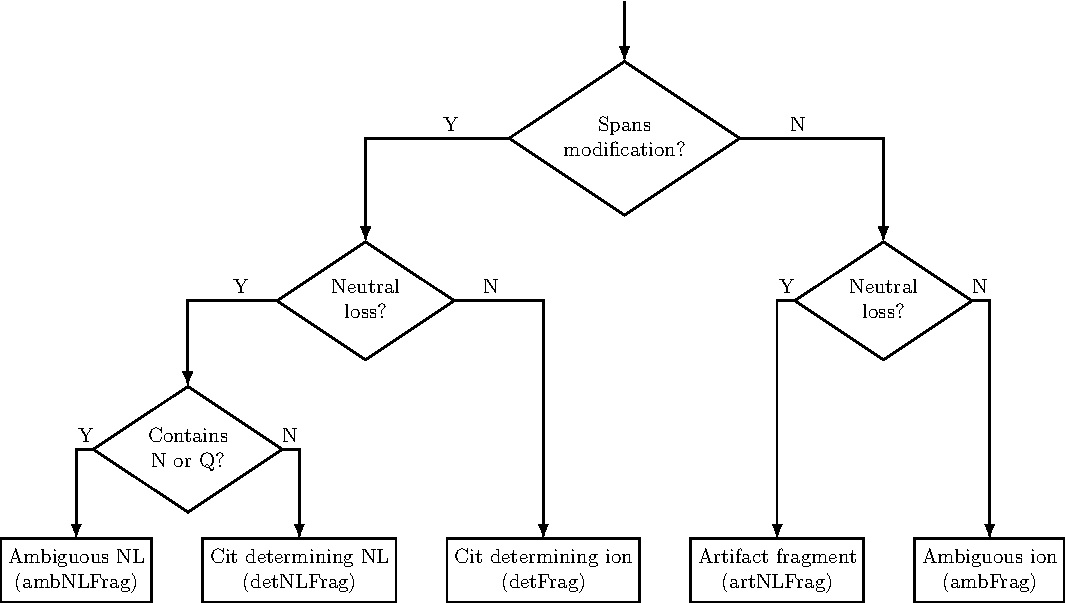
\includegraphics[width=\textwidth]{ionType_decision_tree.pdf}
		\caption{Decision tree for classifying fragment ion type}
		\label{fig:ionType_tree}
	\end{figure}

	\begin{figure}[h!]
		\centering
		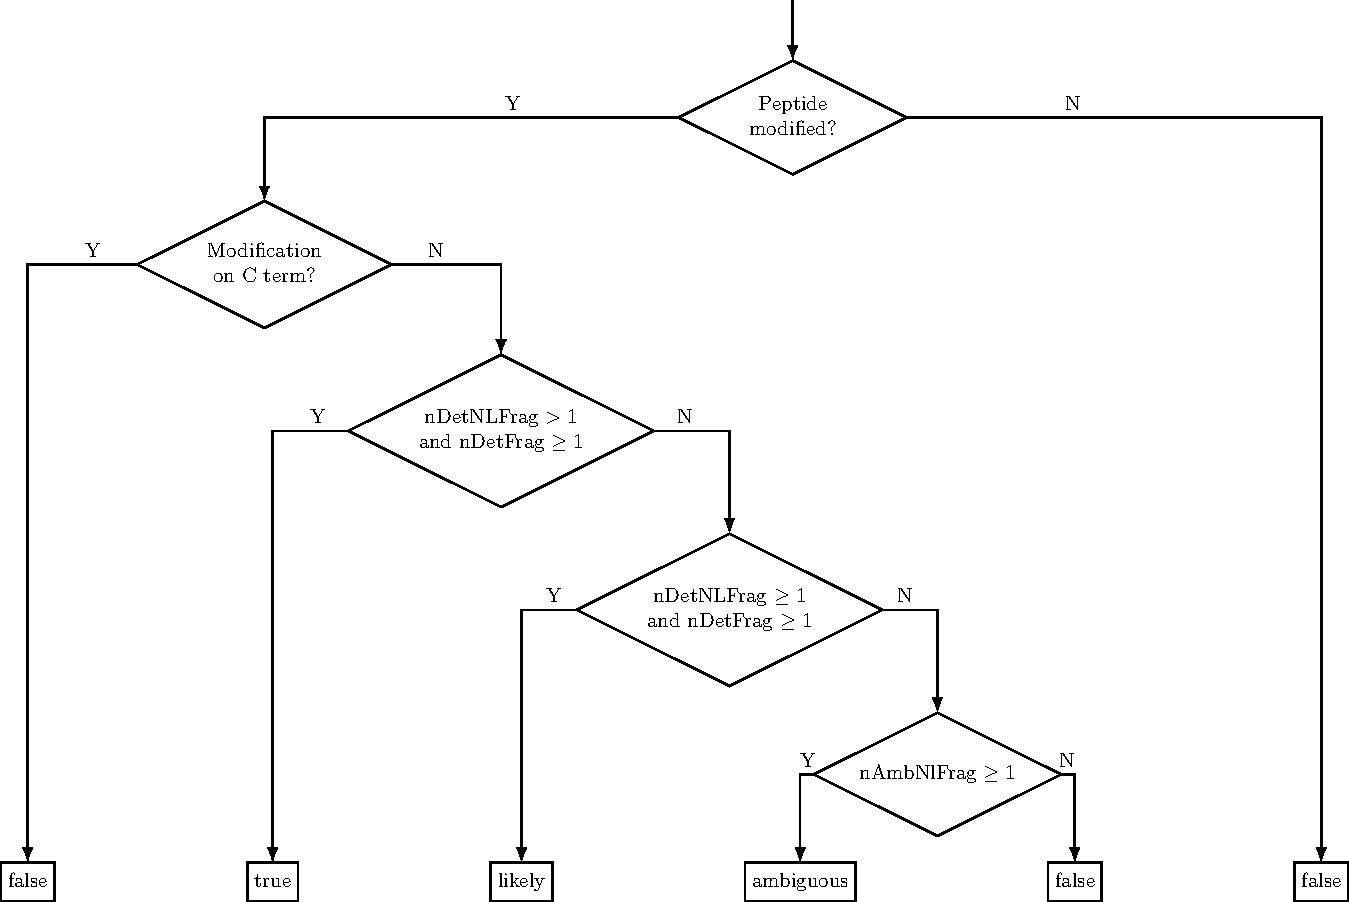
\includegraphics[width=\textwidth]{containsCit_decision_tree.pdf}
		\caption{Decision for determining whether a peptide contains citrulline.}
		\label{fig:containsCit_tree}
	\end{figure}
	
	% section citfinder_program_outline (end)

\end{document}